\section{State of the Art}
\label{chap:etatDeLart}

\subsection{The Visual Novel Genre}

The \gls{vn} is a genre of interactive video game that combines narration, visuals, music, and sometimes voice acting. The genre is historically rooted in Japanese culture and has progressively gained visibility in the West, notably through the distribution of certain anime adaptations and the international circulation of interactive narrative works. \parencite{camingue_what_2021}

On a technical level, a \gls{vn} relies on several fundamental mechanics: textual narration that progresses through clicks, static images representing characters and backgrounds, dialogue choices, and a strong emphasis on sound design and the soundtrack. Figure \ref{fig:higurashi_dialogue} illustrates these elements as they appear in \textit{Higurashi When They Cry Hou - Ch.1 Onikakushi}.

\begin{figure}[htbp]
    \centering
    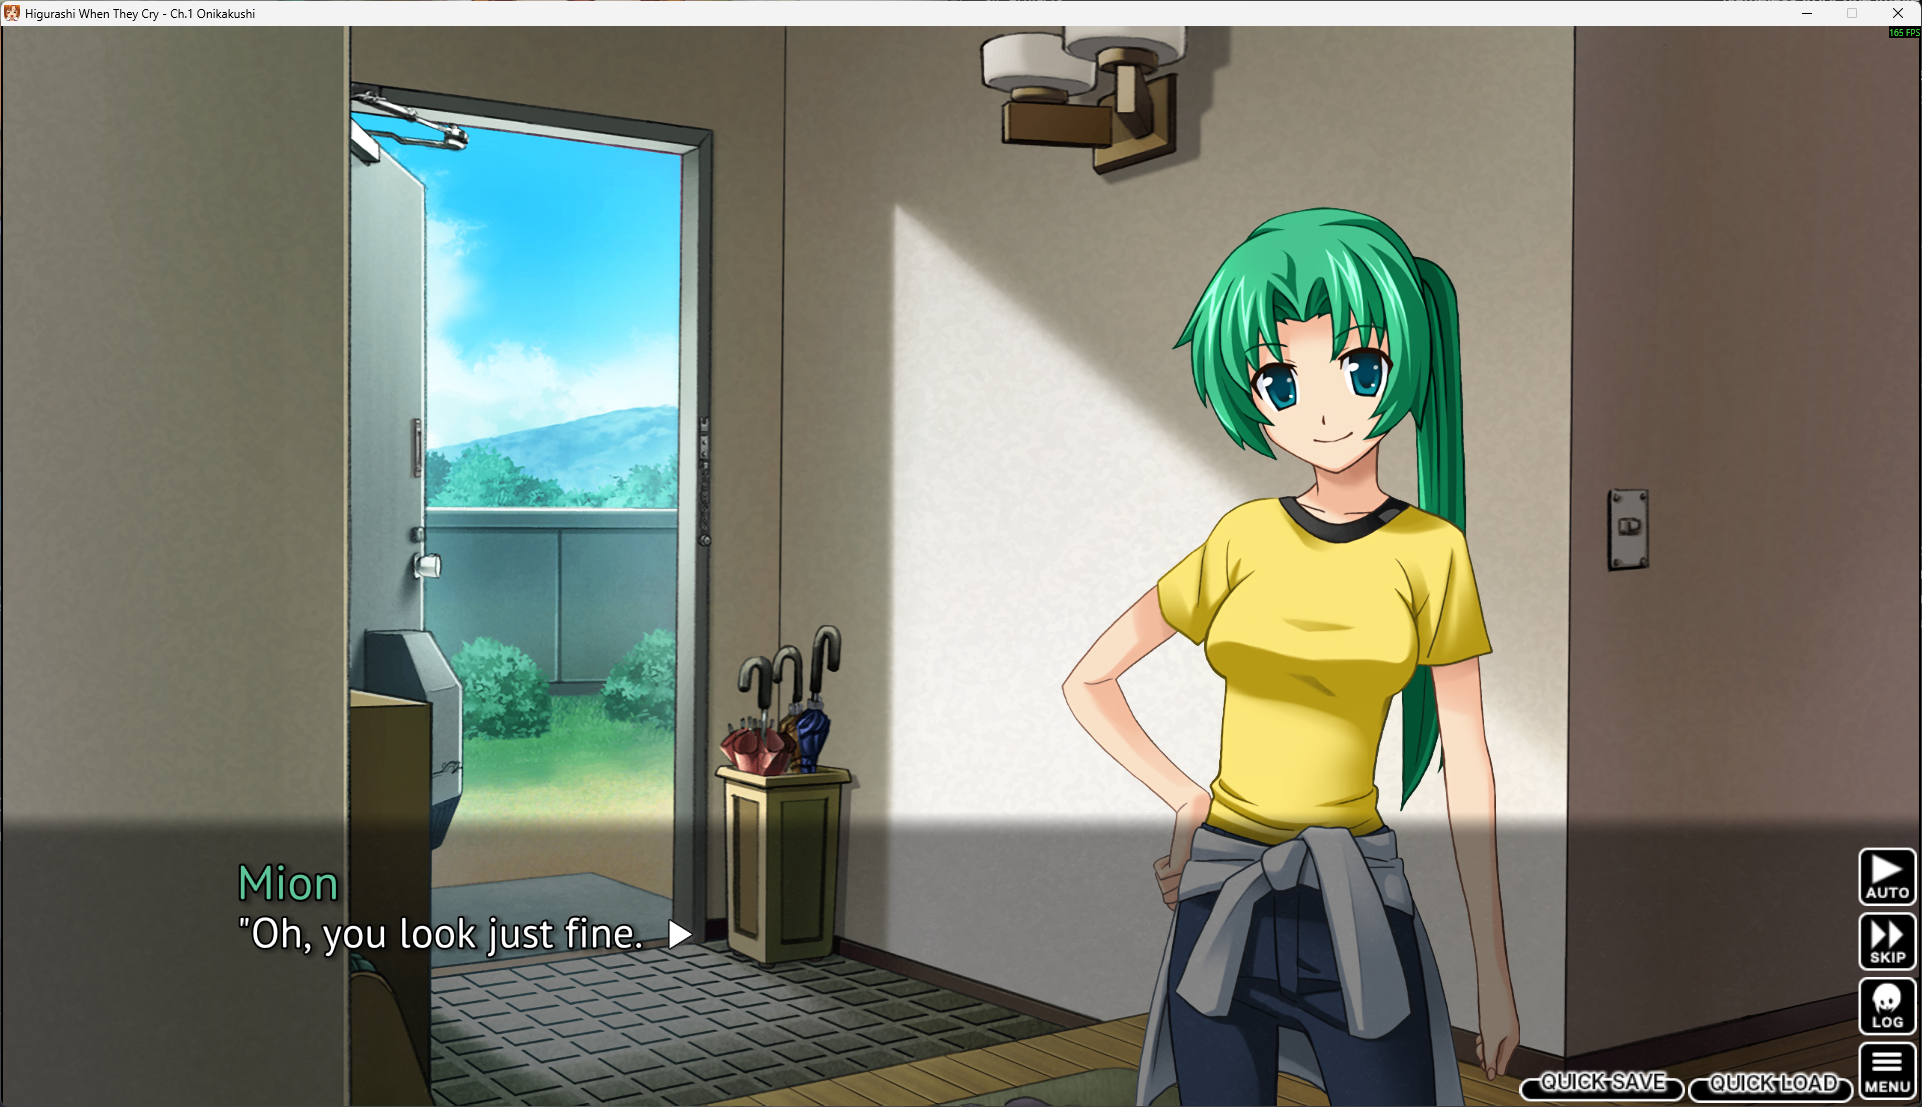
\includegraphics[width=0.9\linewidth]{img/higurashi_dialogue.png}
    \caption{Typical Visual Novel interface: background, character \textit{sprite}, and dialogue box \parencite{07th_expansion_higurashi_2015}}
    \label{fig:higurashi_dialogue}
\end{figure}

Camingue, Carstensdottir, and Melcer found that nine of the thirty academic definitions of the genre mention the presence of branching narration. These structures can lead to very different experiences: \textit{Steins;Gate 0} (2015) offers six different endings, while \textit{428: Shibuya Scramble} (2008) can lead to as many as 95 distinct conclusions. Conversely, 18\% of the titles surveyed contain no narrative branching at all. \parencite{camingue_what_2021}

\clearpage

From a market perspective, the 2019-2024 period saw growth in the genre's popularity, driven by the rise of distribution platforms such as Steam and mobile app stores. On Steam, 17,446 games in the genre are listed in Switzerland\footnote{Number recorded directly on Steam in Switzerland on 29 April 2026 at 19:00.}; the genre enjoys a significant presence there, confirming the existence of an active market. According to a report by Verified Market Research, the global \gls{vn} market was valued at 139 million dollars in 2023 and is expected to reach 620 million dollars by 2031, representing a compound annual growth rate of 8.5\% over the 2024-2031 period. \parencite{noauthor_visual_nodate}

The scale of the genre is also reflected in the count kept by VNDB, a community-run database dedicated to \glspl{vn}. The platform currently lists 64,577 \glspl{vn}\footnote{Number recorded directly on vndb.org on 13 July 2026 at 01:20.}, covering both commercial productions and free or amateur works, on which 52,804 professionals (writers, directors, composers, among others) have been credited\footnote{Number recorded directly on vndb.org on 13 July 2026 at 01:20.}. VNDB also brings together a community of more than 632,000 registered users\footnote{Calculated from the pagination of the site's user list (6,327 pages of 100 users and 21 users on the last page), recorded on 13 July 2026 at 01:20.}. \parencite{vndb_visual_nodate}



\subsection{Existing Visual Novel Engines}
\label{sec:moteur_vn_existant}

Game engines are software tools designed to facilitate game creation, handling recurring technical aspects such as display, resource management, or interaction logic. In the \gls{vn} field, several such tools exist, each based on a different approach to interactive narration.



\subsubsection{Ren'Py}

Several \gls{vn} engines exist. Ren'Py is a \gls{vn} engine used by thousands of creators around the world, allowing interactive stories combining text, images, and sound to be told, on both computer and mobile. To date, Ren'Py has been used to create more than 8,000 \glspl{vn}, games, and other interactive works. \parencite{noauthor_renpy_nodate}

Ren'Py notably offers support for branching narratives, a save system, the ability to roll back within the story, a variety of scene transitions, video playback, and full interface customisation through its dedicated language, \textit{Screen Language}. Ren'Py scripts use a \gls{syntaxe} close to a screenplay format, while also allowing Python blocks to be included for users who want to add advanced features. \parencite{noauthor_renpy_nodate}

\clearpage

Kretzschmar and Raffel argue that Ren'Py's popularity stems from being free of charge, its \glsit{opensource} nature, and the extent of its documentation, which allows anyone to learn its finer points. \parencite{kretzschmar_history_2023}

However, Ren'Py has several limitations for the purposes of this project. Although the engine offers a web export option based on \gls{webassembly}, this feature requires a compilation step through the software's interface, followed by manually uploading the generated files to a compatible host. In addition, the engine's official documentation flags significant restrictions tied to this export: no support for \textit{multi-threading}\footnote{\textbf{Multi-threading}: a program's ability to execute several instruction sequences in parallel, on separate processor cores. \parencite{noauthor_javascript_2026}}, no ability to make network requests from the browser, and file-size constraints imposed by hosting providers. \parencite{noauthor_renpy_nodate}



\subsubsection{Twine}

Twine is a free, open tool for creating non-linear interactive stories in hypertext form: the author links fragments of text, called passages, by means of links, with no programming knowledge required for this basic structure. \parencite{klimas_introduction_nodate}

This approach differs from that of the \gls{vn} engines presented above. Where Ren'Py or the engine developed in this project rely on a script or \gls{schema} file that linearly describes scenes, characters, and dialogue, Twine organises the narrative as a graph of interconnected passages, a structure closer to text-based interactive fiction than to a \gls{vn} in the strict sense, which implies visual staging (backgrounds, \glspl{sprite}, dialogue box). To go beyond a simple hyperlink, for instance to handle variables or conditional logic, the author must use the macro language specific to the chosen story format, which represents an additional learning step compared with simply creating links. \parencite{klimas_introduction_nodate}

Twine is thus a relevant point of comparison for this project: like \nsit, the tool runs in the browser and allows a story to be published as a self-contained file, with no compilation step imposed on the author. It differs, however, in its model for structuring the narrative, based on the hyperlink rather than a declarative data \gls{schema}, and in the absence of integrated visual staging comparable to that of a \gls{vn}.

\clearpage


\subsection{No-code/Low-code Approaches}

\textit{\glsdisp{nocode}{No-code}} platforms allow applications to be created with no programming knowledge, through visual tools, predefined templates, and ready-to-use logic blocks. \textit{\glsdisp{nocode}{Low-code}} tools, on the other hand, allow code to be added for greater control, while remaining accessible to non-developers.

Concretely, \textit{\glsdisp{nocode}{no-code}} platforms rely on drag-and-drop interfaces, prefabricated resources, and visual scripting. \textit{GDevelop}, \textit{Buildbox}, and \textit{Construct} can be cited as representative examples. \textit{\glsdisp{nocode}{Low-code}} tools, such as \textit{Unity's Bolt}, \textit{Unreal Engine's Blueprints}, or \textit{GameMaker Studio}, offer templates and simplified scripting options, with greater flexibility. \parencite{labs_rise_2024}

These approaches are of growing interest in the independent video game industry. Low production costs and the accessibility of development tools have allowed many independent developers to enter the market, leading to an increase in the number of diverse and innovative titles. \parencite{noauthor_visual_nodate}

However, these tools remain mostly tied to graphical interfaces and desktop environments. Writing a story directly as structured text, without going through a visual interface, remains an approach that is little explored in the current ecosystem.



\subsection{Data Description Formats: Comparison and Choice}

To meet the goal of an entirely text-based creation process, the choice of data format is decisive. Several text-based formats are used today to structure data that is readable by humans and interpretable by a machine.


\subsubsection{YAML}

\gls{yaml} is an indentation-based format, known for its readability. However, this readability comes at a cost: its \gls{syntaxe} is sensitive to spacing and special characters, which can produce silent errors that are difficult for a non-developer user to diagnose. In addition, native \glspl{parseur} for \gls{yaml} are not built into web browsers, which would require adding an external dependency to the project. \parencite{noauthor_-_nodate}

\clearpage


\subsubsection{TOML}

\gls{toml} is a format designed for configuration files, clear and explicit in its \gls{syntaxe}. It is, however, less suited to representing the deep hierarchical structures and nested arrays characteristic of a branching scenario. \parencite{noauthor_toml_nodate}


\subsubsection{Ink}

Ink, developed by Inkle Studios, is a narrative scripting language specifically designed for interactive fiction. Its \gls{syntaxe} is expressive and close to natural language, which makes it appealing to authors. However, it requires a dedicated execution engine (the Inkle \glsit{runtime}), which adds an external dependency, and its structure remains a full-fledged programming language, learning which goes beyond the scope of a simple data format. \parencite{noauthor_ink_nodate}


\subsubsection{JSON}

\gls{json} is an open file and data-interchange format that uses human-readable text to store and transmit data objects as key-value pairs and arrays. Although derived from \gls{js}, \gls{json} is independent of any programming language: most modern languages include native tools for generating and parsing data in \gls{json} format. \parencite{noauthor_what_nodate}

For this project, \gls{json} offers several advantages. Its key-value \gls{syntaxe} is intuitive, readable in any text editor, and requires no specialised tool to write. It is thus a natural choice for allowing an author, even without advanced technical skills, to describe a story in a structured way. In addition, \gls{json} is natively supported by \gls{js} and is therefore directly interpretable in a browser with no additional dependency, unlike \gls{yaml} or Ink.

An inherent risk with \gls{json} lies in its sensitivity to \gls{syntaxe} errors: a missing comma or an unclosed quotation mark makes the file invalid. This risk is mitigated in this project by the use of the \gls{zod} \gls{librairie}, which allows not only the file's \gls{syntaxe} but also the conformance of its structure to the \gls{schema} expected by the engine to be validated at runtime, with explicit error messages.